\mysection[Salmon]{Statistik}

\mysubsection{Statistische Grundideen}

\DEF{Deskriptive Statistik}{Graphische Aufbereitung der Daten.}

\DEF{Induktive Statistik}{\begin{enumerate}
    \item Wir erhalten Daten $x_1,...,x_n$ und fassen diese als Realisierungen $X_1(\omega),...,X_n(\omega)$ von ZV $X_1,...,X_n$ auf.
    \item Unter geeigneten Zusatzannahmen suchen wir nach Aussagen über die Verteilung von $X_1,...,X_n$.
\end{enumerate}}

\DEF{Terminologie}{Die Gesamtheit der Beobachtungen $x_1,...,x_n$ oder Zufallsvariablen $X_1,...,X_n$ nennt man oft eine Stichprobe. Die Anzahl $n$ heisst dann der Stichprobenumfang.}

\DEF{Parameterraum}{Ausgangspunkt ist ein Datensatz $x_1,...,x_n$ aus einer Stichprobe $X_1,...,X_n$ für die wir ein Modell suchen.

\begin{enumerate}
    \item Das Modell ist beschreibbar duch einen (mögl'weise hochdimensionalen) Parameter $\vartheta$ aus dem Parameterraum $\Theta$.
    \item Wir betrachten simultan eine ganze Familie von Wahr'räumen $(\Omega,\mathcal{F},\P_{\vartheta})_{\vartheta\in\Theta}$. \begin{enumerate}
        \item Man hat typisch einen festen Grundraum $(\Omega,\mathcal{F})$, und
        \item ein $\P_{\vartheta}$ auf $(\Omega,\mathcal{F})\ \forall\ \vartheta\in\Theta$.
    \end{enumerate}
    \item Das finden von $\vartheta$ und ein passendes Modell für gegebene Daten, nennt man parametrische statistische Analyse. 
\end{enumerate}}

\DEF{Parametrische Statistische Analyse}{
\begin{enumerate}
    \item \textbf{Deskriptive Statistik:} Mit graphischen Methoden eine erste Idee für die Wahl ener geeigneten Modellierung zu finden.
    \item \textbf{Wahl eines (parametrischen) Modells:} Spezifizieren der Parametermenge und der Familie $(\P_{\vartheta})_{\vartheta\in\Theta}$ von Modellen, mit denen man arbeiten will.
    \item \textbf{Schätzung der Parameter:} Möglichst gut passendes Modell unter Benutzung eines Schätzers wählen. Die zugehörige Schätzfunktion ist eine Abbildung, die gegebenen Daten $x_1,...,x_n$ ein $\vartheta\in\Theta$ zuordnet.
    \item \textbf{Kritische Modellüberprüfung (Anpassungstest):} Überprüfen, wie gut der Parameter $\vartheta$ bzw. das Modell $\P_{\vartheta}$ zu den Daten passen, unter Verwendung statistischer Tests.
    \item \textbf{Assagen über Zuverlässigkeit der Schätzungen:} Man kann auch versuchen, einen Bereich in $\Theta$ so zu spezifizieren, dass alle zughörigen Modelle $\P_{\varepsilon}$ in einem zu präzisierenden Sinn gut zu den Daten passen. Man spricht dann avon einen Konfidenzbereich. 
\end{enumerate}}


\mysubsection{Schätzer}

\DEF{Schätzer}{Eine ZV der Form $T_l=t_l(X_1,...,X_n)$. Die Schätzfunktionen $t_l:\R^n\rightarrow\R$ müssen noch gewählt werden.

Einsetzen von Daten $x_k=X_k(\omega),k=1,...,n,$ liefert dann Schätzwerte (sample estimates) $T_l(\omega)=t_l(x_1,...,x_n)$ für $\vartheta_l,l=1,...,m$.

Der kürze halber schreiben wir oft $T=(T_1,...,T_m)$ und $\vartheta=(\vartheta_1,...,\vartheta_m)$.}

\DEF{Erwartungstreue}{Ein Schätzer $T$ heisst erwartungstreu (unbiased) für $\vartheta$, falls $\forall\vartheta\in\Theta:\E_{\vartheta}[T]=\vartheta$.

Interpretation: Im Mittel (über alle denkbaren Realisierungen $\omega$) schätzt $T$ also richtig, und zwar unabhängig davon, welches Modell $\P_{\vartheta}$ zu Grunde liegt.}

\DEF{Bias und MSE}{Sei $\vartheta\in\Theta$ und $T$ ein Schätzer.
\begin{enumerate}
    \item Der Bias (erwartete Schätzfehler) von $T$ im Modell $\P_{\vartheta}$ ist definiert als $\E_{\vartheta}[T]-\vartheta$.
    \item MSE von $T$ im Modell $\P_{\vartheta}$ ist definiert als $MSE_{\vartheta}[T]=\E_{\vartheta}[(T-\vartheta)^2]$.
    \item Eine Folge von Schätzern $T^{(n)},n\in\N$, heisst konsistent für $\vartheta$, falls $T^{(n)}$ für $n\rightarrow\infty$ in $\P_{\vartheta}-$Wahr' gegen $\vartheta$ konvergiert $\Leftrightarrow$ $\forall\vartheta\in\Theta,\forall\varepsilon >0:\lim_{n\rightarrow\infty}\P_{\vartheta}[|T^{(n)}-\vartheta|>\varepsilon]=0$.
\end{enumerate}}

\NOTE{7.7}{$MSE_{\vartheta}[T]=\E_{\vartheta}[(T-\vartheta)^2]=\V_{\vartheta}[T]+(\E_{\vartheta}[T]-\vartheta)^2$ $\Rightarrow$ $T$ erwartungstreu $\Leftrightarrow$ $MSE_{\vartheta}[T]=\V_{\vartheta}[T]$.}


\mysubsection{Maximum-Likelihood-Methode}

\DEF{Notation}{In jedem Modell $\P_{\vartheta}$ sind $(X_1,...,X_n)$ entweder
\begin{enumerate}
    \item diskret mit gemeinsamer Gewichtsfunktion $p_{\substack{\rightarrow\\ X}}(x_1,...,x_n;\vartheta)$, oder
    \item stetig mit gemeinsamer Dichtefunktion $f_{\substack{\rightarrow\\ X}}(x_1,...,x_n;\vartheta)$.
\end{enumerate}

Meistens sind die $X_k$ unter $\P_{\vartheta}$ sogar i.i.d. mit individueller $p_X(x;\vartheta)$ bzw. $f_X(x;\vartheta)$. Somit gilt
\begin{enumerate}
    \item $p_{\substack{\rightarrow\\ X}}(x_1,...,x_n;\vartheta)=\prod_{k=1}^np_X(x_k;\vartheta)$,
    \item $f_{\substack{\rightarrow\\ X}}(x_1,...,x_n;\vartheta)=\prod_{k=1}^nf_X(x_k;\vartheta)$.
\end{enumerate}

Weiter gilt $p_{\substack{\rightarrow\\ X}}(x_1,...,x_n;\vartheta)=\P_{\vartheta}[X_1=x_1,...,X_n=x_n]$ und $f_{\substack{\rightarrow\\ X}}$ ist wie immer das stetige Analogon.}

\DEF{Likelihood-Funktion}{$L(x_1,...,x_n;\vartheta)=\begin{cases}
    p_{\substack{\rightarrow\\ X}}(x_1,...,x_n;\vartheta) & \text{im diskreten Fall,}\\
    f_{\substack{\rightarrow\\ X}}(x_1,...,x_n;\vartheta) & \text{im stetigen Fall.}
\end{cases}$}

\DEF{Log-Likelihood-Funktion}{$log(L(x_1,...,x_2;\vartheta))$ wobei $log=ln$. Hat im i.i.d.-Fall den Vorteil durch eine Summe gegeben zu sein.}

\DEF{ML-Schätzer}{$T_{ML}$ für $\vartheta$ wird dadurch definiert, dass er $\vartheta\mapsto L(X_1,...,X_n;\vartheta)$ über alle $\vartheta$ maximiert. Also $T_{ML}=t_{ML}(X_1,...,X_n)\in argmax_{\vartheta\in\Theta}L(X_1,...,X_n;\vartheta)$.}

\EXAMPLE{ML-Schätzer für Bernoulli-Verteilung}{Sei $\vartheta=p$. Im Modell $\P_p$ seien $X_1,...,X_n\  \text{i.i.d.}\ \sim Ber(p)$. Dann $p_X(x;\vartheta)=\P_{\vartheta}[X=x]=\vartheta^x(1-\vartheta)^{1-x}$ für $x\in\{0,1\}$. Da $X_k$ i.i.d. folgt 
\begin{align*}
L(x_1,...,x_n;\vartheta)&=\prod_{k=1}^np_X(x_k;\vartheta)\\&=\vartheta^{\sum_{k=1}^nx_k}(1-\vartheta)^{n-\sum_{k=1}^nx_k}
\end{align*}
und
\begin{align*}
&log(L(x_1,...,x_n;\vartheta))=\\&log(\vartheta)\sum_{k=1}^nx_k+log(1-\vartheta)(n-\sum_{k=1}^nx_k).
\end{align*}

Leiten wir nach $\vartheta$ ab erhalten wir
\begin{align*}
    \frac{\partial}{\partial\vartheta}log(L(x_1,...,x_n;\vartheta))=\frac{1}{\vartheta}\sum_{k=1}^nx_k-\frac{1}{1-\vartheta}(n-\sum_{k=1}^nx_k).
\end{align*}

Weiter folgt
\begin{align*}
        \frac{\partial}{\partial\vartheta}log(L(x_1,...,x_n;\vartheta))=0
\end{align*}
\begin{align*}
    \Leftrightarrow
\end{align*}
\begin{align*}
    (1-\vartheta)\sum_{k=1}^nx_k=\vartheta(n-\sum_{k=1}^nx_k)
\end{align*}
\begin{align*}
    \Leftrightarrow
\end{align*}
\begin{align*}
    \vartheta=\frac{1}{n}\sum_{k=1}^nx_k.
\end{align*}

Der ML-Schätzer für $\vartheta$ bzw. $p$ ist hier also 
\begin{align*}
    T=\frac{1}{n}\sum_{k=1}^nX_k=\overline{X}_n.
\end{align*}}

\EXAMPLE{ML-Schätzer für Geom'-Verteilung}{Seien $X_1,...,X_n\  \text{i.i.d.}\ \sim Geom(\vartheta)$. Dann 
\begin{enumerate}
    \item $L(x_1,...,x_n;\vartheta)=\vartheta^n(1-\vartheta)^{x_1+...+x_n-n}$.
    \item $T_{ML}=\frac{n}{\sum_{i=1}^nX_i}$.
\end{enumerate}}

\EXAMPLE{ML-Schätzer für Normal-Verteilung}{Seien $X_1,...,X_n\  \text{i.i.d.}\ \sim \mathcal{N}(\mu,\sigma^2)$ wobei $\vartheta=(\mu,\sigma^2)=(u,v)$. Also $T=(T_1,T_2)$. Siehe Example 8.12 für Likelihood-Funktion.
\begin{enumerate}
    \item $T_1=\overline{X}_n$.
    \item $T_2=\frac{1}{n}\sum_{i=1}^nX_i^2-(\overline{X}_n)^2$.
\end{enumerate}

Achtung, $T_2$ ist nicht erwartungstreu. Erwartungstreue Version ist:
\begin{enumerate}
    \item $T_1'=\overline{X}_n$.
    \item $T_2'=\frac{1}{n-1}\sum_{i=1}^n(X_i-\overline{X}_n)^2=:S^2$.
\end{enumerate}}

\EXAMPLE{ML-Schätzer für Exp-Verteilung}{Seien $X_1,...,X_n\  \text{i.i.d.}\ \sim Exp(\vartheta)$. Dann 
\begin{enumerate}
    \item $L(x_1,...,x_n;\vartheta)=\vartheta^ne^{-\vartheta(x_1+...+x_n)}$.
    \item $T_{ML}=\frac{n}{\sum_{i=1}^nX_i}$.
\end{enumerate}}

\mysubsection{Verteilungsaussagen}

\DEF{$\chi^2-$Verteilung}{Sei $X$ stetige ZV. Falls für $x\geq 0:$ $f_X(x)=\frac{1}{2^\frac{m}{2}\Gamma(\frac{m}{2})}x^{\frac{m}{2}-1}e^{-\frac{x}{2}}$ $\Rightarrow X\sim\chi_m^2$ $\Leftrightarrow X$ ist $\chi^2$-verteilt mit $m$ Freiheitsgraden.
\begin{enumerate}
    \item Entstehung: Sind ZV $X_1,...,X_m$ i.i.d. $\sim\mathcal{N}(0,1)$. Dann $\sum_{k=1}^mX_k^2\sim\chi_m^2$. Also $\E[X]=\E[X_1^2]+...+\E[X_m^2]=m$.
    \item $\chi_m^2-$Verteilung ist ein Spezialfall einer $Ga(\alpha,\lambda)-$Verteilung mit $\alpha=\frac{m}{2},\lambda=\frac{1}{2}$.
    \item Wählt man $m=2$ erhält man eine Exponentialverteilung mit Parameter $\lambda=\frac{1}{2}$.
\end{enumerate}}
\begin{figure}[H]
 \centering
 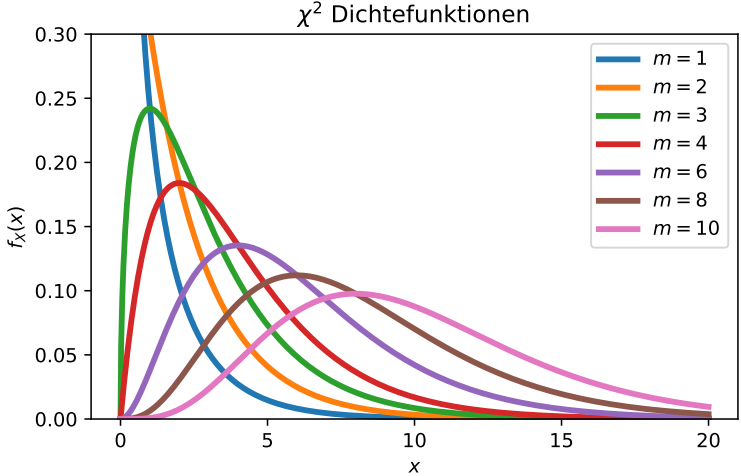
\includegraphics[width=\linewidth,keepaspectratio]{pictures/chi_squared_pdf.png} 
\end{figure}


\DEF{Gammafunktion}{$x\geq 0:\Gamma(x)=\int_0^{\infty}t^{x-1}e^{-t}dt$. Es gilt $\Gamma(n+1)=n!$ für $n\in\N_0$.}

\DEF{Studentsche t-Verteilung}{Sei $X$ stetige ZV. Falls für $x\in\R:$ $f_X(x)=\frac{\Gamma(\frac{m+1}{2})}{\sqrt{m\pi}\Gamma(\frac{m}{2})}(1+\frac{x^2}{m})^{-\frac{m+1}{2}}$ $\Rightarrow X\sim t_m$ $\Leftrightarrow X$ ist $t$-verteilt mit $m$ Freiheitsgraden.
\begin{enumerate}
    \item Entstehung: Sind $X\sim\mathcal{N}(0,1), Y\sim\chi_m^2$ unabhängig $\Rightarrow$ $\frac{X}{\sqrt{\frac{1}{m}Y}}\sim t_m$.
    \item Für $m=1$ erhält man eine Cauchy-Verteilung.
    \item Für $m\rightarrow\infty$ erhält man eine $\mathcal{N}(0,1)$-Verteilung.
    \item Ähnlich wie $\mathcal{N}(0,1)$ aber langschwänziger (long-tailed).
\end{enumerate}}
\begin{figure}[H]
 \centering
 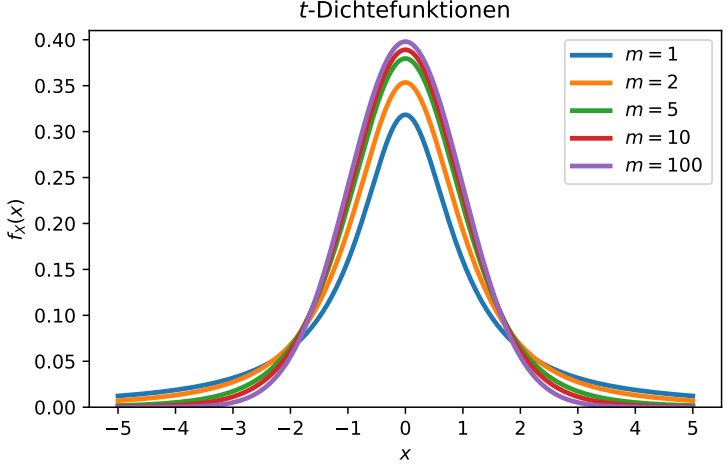
\includegraphics[width=\linewidth,keepaspectratio]{pictures/t_distribution_pdf.png} 
\end{figure}

\SA{7.20}{Seien $X_1,...X_n$ i.i.d. $\sim\mathcal{\mu,\sigma^2}$ und \begin{align*}
\overline{X}_n=\sum_{k=1}^n,\hspace{10px}S^2=\frac{1}{n-1}\sum_{k=1}^n(X_k-\overline{X}_n)^2.
\end{align*}

Es gelten folgende Aussagen:
\begin{align*}
    &1.\ \overline{X}_n\sim\mathcal{N}(\mu,\frac{1}{n}\sigma^2)\Leftrightarrow\frac{\overline{X}_n-\mu}{\frac{\sigma}{\sqrt{n}}}\sim\mathcal{N}(0,1),\\
    &2.\ \frac{n-1}{\sigma^2}S^2=\frac{1}{\sigma^2}\sum_{k=1}^n(X_k-\overline{X}_n)^2\sim\chi_{n-1}^2,\\
    &3.\ \overline{X}_n\ \text{und}\ S^2\ \text{sind unabhängig},\\
    &4.\ \frac{\overline{X}_n-\mu}{\frac{S}{\sqrt{n}}}=\frac{\frac{\overline{X}_n-\mu}{\sigma/\sqrt{n}}}{S/\sigma}=\frac{\frac{\overline{X}_n-\mu}{\sigma/\sqrt{n}}}{\sqrt{\frac{1}{n-1}\frac{n-1}{\sigma^2}S^2}}\sim t_{n-1}.
\end{align*}}
